% chapter03.tex

 %%%%%%%%%%%%%%%%%%%%%%%%%%%%%%%%%%%%%%%%%%%%%%%%%%%%%%%%%%%%%%%%%%%%%%%%%%%%%
 %                                                                           %
 %    PyMS documentation                                                     %
 %    Copyright (C) 2005-8 Vladimir Likic                                    %
 %                                                                           %
 %    The files in this directory provided under the Creative Commons        %
 %    Attribution-NonCommercial-NoDerivs 2.1 Australia license               %
 %    http://creativecommons.org/licenses/by-nc-nd/2.1/au/                   %
 %    See the file license.txt                                               %
 %                                                                           %
 %%%%%%%%%%%%%%%%%%%%%%%%%%%%%%%%%%%%%%%%%%%%%%%%%%%%%%%%%%%%%%%%%%%%%%%%%%%%%

\chapter{GC-MS data derived objects}

In this chapter the methods for converting the raw GC-MS data to an
Intensity Matrix object are illustrated.

In the raw GC-MS data, consecutive scans do not necessarily contain the same
mass per charge (mass) values. For data processing, it is often necessary to
convert the data to a matrix with a set number of masses and scans. In PyMS
there are functions to explicitly convert the raw mass values to consistent
values across all scans.

\section{IntensityMatrix Object}

The general scheme for converting raw mass values is to bin intensity values
based on the interval the corresponding mass belongs to. The general procedure
is as follows:
\begin{itemize}
    \item for a given bin size
    \item calculate the number of bins to cover the range of all masses.
    \item centre the first bin at the minimum mass found for all the raw data.
    \item sum intensities whose masses are in a given bin.
\end{itemize}

A mass, $m$, is considered to belong to a bin when
$c - w/2 \le m < c + w/2$
, where $c$ is the centre of the bin, and $w$ is
the width of the bin.

A function to bin masses to the nearest integer is also available.

% Figure~\ref{fig:binning} illustrates the process of assigning bins to the mass
% axis and summing all intensities in a given bin. The result is a new mass axis
% with mass values corresponding to the centre of each bin.

% \begin{figure}[htp]
% \begin{center}
% %\includegraphics{graphics/binning/binning.eps}
% \caption{Mass intensity values are added to bins based on a pre-set bin size
%and
% the minimum mass of all the scan data. All intensities in a given bin width
% (top) are added and given a mass of the centre of the bin (bottom). For
%integer
% binning, each bin has a width of one and is centred at integer values.}
% \label{fig:binning}
% \end{center}
% \end{figure}

\noindent
[ {\em This example is in pyms-test/30} ]

An intensity matrix on the raw GCMS data can be built using the following
functions. First the raw data is imported as before.

\begin{verbatim}
>>> from pyms.GCMS.IO.JCAMP.Function import JCAMP_reader
>>> jcamp_file = "/x/PyMS/data/gc01_0812_066.jdx"
>>> data = JCAMP_reader(jcamp_file)
 -> Reading JCAMP file '/x/PyMS/pyms-data/gc01_0812_066.jdx'
>>>
\end{verbatim}

\noindent
Then the data can be converted to an intensity matrix using the functions
available in ``pyms.GCMS.Functions'', namely {\tt build\_intensity\_matrix()}
and {\tt build\_intensity\_matrix\_i()}.

The default operation of {\tt build\_intensity\_matrix()} is to use a bin size
of one and treat the masses as floating point numbers. The default intensity
matrix can be built as follows:

\begin{verbatim}
>>> from pyms.GCMS.Function import build_intensity_matrix
>>> im = build_intensity_matrix(data)
\end{verbatim}

The size as the number of scans and the number of bins is returned by:
\begin{verbatim}
>>> im.get_size()
\end{verbatim}

There are 9865 scans, 551 bins in this example.

The raw masses have been binned into new mass units based on the minimum mass
in the raw data and the bin size. A list of the new masses are returned by:

\begin{verbatim}
>>> masses = im.get_mass_list()
\end{verbatim}

It is also possible to search for a particular mass, by finding the index of the
binned mass closest to the desired mass. For example, the index of the closest
binned mass to a mass of 73.3 m/z is returned by:

\begin{verbatim}
>>> index = im.get_index_of_mass(73.3)
\end{verbatim}

The value of the closest mass can be returned by indexing into the mass list:
\begin{verbatim}
>>> print masses[index]
\end{verbatim}

A mass of 73.0 is returned in this example.

The bin size can be set values other than one. For example, the bin size can be
set to 0.5.

\begin{verbatim}
im = build_intensity_matrix(data, 0.5)
\end{verbatim}

The size of the intensity matrix will reflect the change in the number of bins.
\begin{verbatim}
>>> im.get_size()
\end{verbatim}

There are 9865 scans (as before) and 1101 bins in this example.

The index and binned mass of the mass closest to 73.3 should also reflect the
different binning.
\begin{verbatim}
>>> masses = im.get_mass_list()
>>> index = im.get_index_of_mass(73.3)
>>> print masses[index]
\end{verbatim}

A mass of 73.5 is returned in this example.

It is also possible to build an intensity matrix with masses rounded to the
nearest integer using a bin size of one. The function is imported from
``pyms.GCMS.Functions''.
\begin{verbatim}
>>> from pyms.GCMS.Function import build_intensity_matrix_i
>>> im = build_intensity_matrix_i(data)
\end{verbatim}

The masses are now all integers.
\begin{verbatim}
>>> masses = im.get_mass_list()
>>> index = im.get_index_of_mass(73.3)
>>> print masses[index]
\end{verbatim}

A mass of 73 is returned in this example.

\section{MassSpectrum Object}

\noindent
A MassSpectrum object contains two attributes, {\tt mass\_list} and
{\tt mass\_spec}, a list of the mass values and corresponding intensities,
respectively. MassSpectrum is returned by the IntensityMatrix method of {\tt
get\_ms\_at\_index(index)}.

\section{IonChromatogram Object}

\noindent
An IonChromatogram object is a one dimensional vector containing
mass intensities as a function of retention time. This can can be either
m/z channel intensities (for example, ion chromatograms at m/z = 65),
or cumulative intensities over all measured m/z (TIC).

An ion chromatogram object has a method {\tt is\_tic()} which returns
True is the ion chromatogram is TIC, False otherwise:

\begin{verbatim}
>>> print "'tic' is a TIC:", tic.is_tic()
'tic' is a TIC: True
>>> print "'ic' is a TIC:",ic.is_tic()
'ic' is a TIC: False
\end{verbatim}

\subsection{Writing data to a file}

The method {\tt write()} of IonChromatogram object allows one to save
the ion chromatogram object to a file:

\begin{verbatim}
>>> tic.write("output/tic.dat", minutes=True)
>>> ic.write("output/ic.dat", minutes=True)
\end{verbatim}

\noindent
The flag minutes=True indicates that retention time will be saved in minutes.
The ion chromatogram object saved with with the {\tt write{}} method is a
plain ASCII file which contains a pair of (retention time, intensity) per
line.

\begin{verbatim}
$ head tic.dat
  5.0930 2.222021e+07
  5.0993 2.212489e+07
  5.1056 2.208650e+07
  5.1118 2.208815e+07
  5.1181 2.200635e+07
  5.1243 2.200326e+07
  5.1306 2.202363e+07
  5.1368 2.198357e+07
  5.1431 2.197408e+07
  5.1493 2.193351e+07
\end{verbatim}

% \noindent
% Figure \ref{fig:tic-plot} shows the plot of the file 'tic.dat' produced with
% the program Gnuplot.
%
% \begin{figure}[htp]
% \begin{center}
% %x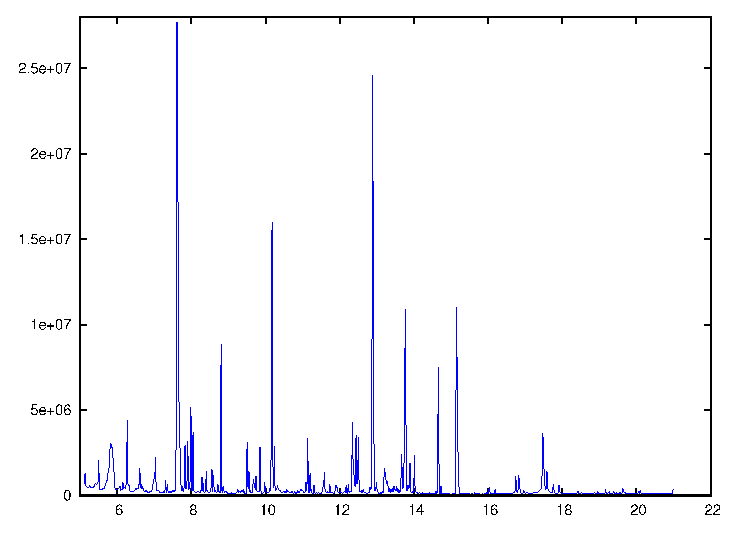
\includegraphics{graphics/pyms-test/tic.eps}
% \caption{The Gnuplot plot of the file 'tic.dat'}
% \label{fig:tic-plot}
% \end{center}
% \end{figure}

\section{Saving data}

\noindent
A matrix of intensity values can be saved to a file with the function
{\tt save\_data()} from {\tt pyms.Utils.IO}. A matrix of intensity values can
be returned from an IntensityMatrix with the method {\tt get\_matrix\_list()}.
For example,

\begin{verbatim}
>>> from pyms.Utils.IO import save_data
>>> mat = im.get_matrix_list()
>>> save_data("output/im.dat", mat)
\end{verbatim}

The entire IntensityMatrix can be saved as CSV with the method
{\tt export\_csv()}. For example,

\begin{verbatim}
>>> im.export_csv("output/data")
\end{verbatim}

\noindent
will create 'data.im.csv, data.mz.csv, and data.rt.csv where these are the
intensity matrix, retention time vector, and m/z vector in the CSV format.

Additionally, the entire IntensityMatrix can be exported as LECO CSV. This is
 useful for import into other analytical software packages.

\begin{verbatim}
>>> im.export_leco_csv("output/data_leco.csv")
\end{verbatim}
